% !TeX spellcheck = en_US

\chapter{Basis}
\label{chap:basis}
In this chapter, the fundamentals used in this work will be explained.
These include definitions for Cloud computing and Cloud applications, description of TOSCA standard and its implementation: OpenTOSCA.
At the end, a package management and tools for its automation are described.
\section{Cloud computing and Cloud application} \label{sec:cloud}
Understanding the problem requires a clear definition of the term "Cloud computing".
%In everyday life, you can often hear the phrase "Cloud computing", but what is it?\\
%\subsection{Definitions}
Unfortunately, a generally accepted definition of Cloud computing that describes all possible situations doesn't exist. 
But in the scientific community, the definition put forward by \gls{nist}~\cite*{wwwnist} is commonly used. 
This definition appropriately describes the concept of Cloud computing used in this paper, and therefore this definition will be used.\\
%\begin{definition}[Cloud computing]
\emph{\textbf{Cloud computing}\label{def:nist} is a model for enabling ubiquitous, convenient, on-demand network access to a shared pool of configurable computing resources (e.g., networks, servers, storage, applications, and services) that can be rapidly provisioned and released with minimal management effort or service provider interaction.}~\cite*{nist}\\
%\end{definition}
But computing is too abstract term, for our purpose we need something more practical, like an application.
Also, the are no generally accepted definitions of Cloud application, but it can be obtained from the definition of Cloud computing.\\
%\begin{definition}[Cloud application] 
\emph{A \textbf{Cloud application}\label{def:capp} is an application that is executed according to the Cloud computing model.} \\%~\cite*{cloudapp}\\
%\end{definition} 
In addition, a short meanings of a Cloud system, a provider, and a user will be provided.\\
%\begin{definition}[Cloud system] 
A composite Cloud application which consist of multiple small applications will be called a \textbf{Cloud system}\label{def:csys}. %\\
%\end{definition} 
%\subsubsection{Sides}
An owner of the physical platform, where Cloud computing takes place is called a \textbf{provider}.
An owner of the Cloud application renting a provider's platform is called a \textbf{user}.
\clearpage
\subsection*{Service Models}\label{def:servmod}
Cloud applications provide a wide range of different services.
Some groups of services which follow the common rules and perform the similar function are described by service models.
NIST distinguishes between three main types of such models.
\begin{itemize}
	\item  \gls{saas}. 
	The capability provided to the consumer is to use the provider’s applications running on a Cloud infrastructure. 
	The applications are accessible from various client devices through either a thin client interface, such as a web browser (e.g., web-based email), or a program interface. 
	The consumer does not manage or control the underlying Cloud infrastructure including network, servers, operating systems, storage, or even individual application capabilities, with the possible exception of limited userspecific application configuration settings.~\cite*{nist}
	\item \gls{paas}. 
	The capability provided to the consumer is to deploy onto the Cloud infrastructure consumer-created or acquired applications created using programming languages, libraries, services, and tools supported by the provider.
	The consumer does not manage or control the underlying Cloud infrastructure including network, servers, operating systems, or storage, but has control over the deployed applications and possibly configuration settings for the application-hosting environment.~\cite*{nist}
	\item \gls{iaas}.
	The capability provided to the consumer is to provision processing, storage, networks, and other fundamental computing resources where the
	consumer is able to deploy and run arbitrary software, which can include operating systems and applications.
	The consumer does not manage or control the underlying Cloud infrastructure but has control over operating systems, storage, and deployed applications; and possibly limited control of select networking components (e.g., host firewalls).~\cite*{nist}
\end{itemize}
%\subsection*{Deployment models}
%Similarly, NIST distinguishes between four types of deployment models.
%\begin{itemize}
%	\item Private cloud. 
%	The cloud infrastructure is provisioned for exclusive use by a single organization comprising multiple consumers (e.g., business units). It may be owned, managed, and operated by the organization, a third party, or some combination of them, and it may exist on or off premises.
%\item Community cloud.
%	The cloud infrastructure is provisioned for exclusive use by a specific community of consumers from organizations that have shared concerns (e.g., mission, security requirements, policy, and compliance considerations).
%	It may be owned, managed, and operated by one or more of the organizations in the community, a third party, or some combination of them, and it may exist on or off premises.
%\item Public cloud.
%	The cloud infrastructure is provisioned for open use by the general public. 
%	It may be owned, managed, and operated by a business, academic, or government organization, or some combination of them.
%	It exists on the premises of the cloud provider.
%\item Hybrid cloud. 
%	The cloud infrastructure is a composition of two or more distinct cloud infrastructures (private, community, or public) that remain unique entities, but are bound together by standardized or proprietary technology that enables data and application portability (e.g., cloud bursting for load balancing between clouds). 
%\end{itemize}
\subsection*{Usage of Cloud Computations}
Nowadays Cloud computing and applications can be found everywhere, and their number constantly grows~\cite*{cloud_stat}.
They are used for test and development, big data analyses, file storage and so on.
Cloud computing allows using resources effectively, to distribute the load to a system from several physical servers and to shift the maintenance to the providers. 
If  a service uses a single physical server and this server will be disabled, then the entire service will be completely unavailable too.
But if a Cloud application uses a hundred of physical servers, then disabling of one will not carry such serious consequences.
In addition, a user doesn't need to maintain a team of administrators for the event of various problems.\\
A user doesn't have a direct access to the infrastructure (servers and operating systems) when using a PaaS or a SaaS service models. He can operate only with the provided Application Programming Interface (API).
An API provides a set of methods to communicate with provider's infrastructure. 
Each provider defines his own set of methods, depending on his area of specialization. 
On the one hand, this specialization makes easier to work with the provider, but on the other hand, it becomes more difficult to redeploy an application to another provider.
\section{Topology and Orchestration Specification for Cloud	Applications} \label{sec:tosca}
%\subsection*{Definition}
The Topology and Orchestration Specification for Cloud Applications (\gls{tosca}) standard developed by \gls{oasis}~\cite{oasis} provides a new way to enable portable automated deployment and management of Cloud applications.
\gls{tosca} describes the structure of an application as a topology containing components and relationships between them.
%Plans capture management tasks by orchestrating management operations exposed by the components. \cite*{INBOOK-2014-01}
\gls{tosca} application is a Cloud application described according to the TOSCA standard.
This standard can be used not only to describe all stages of a Cloud application life-cycle but also to serve as a layer between the Cloud application and provider's API, allowing to implement a single application suitable for working with different providers. 
\subsection*{Structure of TOSCA Applications}
TOSCA specification provides a language to define components (described in section~\ref{def:servmod}) and relationships between them using $Service$ $Templates$. 
In addition it describes the management procedures which create or modify services using orchestration processes.
The description of elements of a TOSCA structure used in this work is provided. \\
A $Service$ $Template$ is the main component in a \gls{tosca} structure. 
It defines the structure (Topology Template) and process models (Plans) of the service. 
There can be many Service Templates within one TOSCA application.
The combination of topology and orchestration in a Service Template defines what is needed to be preserved across deployments in different environments to enable interoperable deployment of Cloud services and their management throughout the complete lifecycle (e.g. scaling, patching, monitoring, etc.).
This is useful when an application is ported to alternative Cloud environments.~\cite{TOSCA-v1.0_book} \\ %\\
$Plans$ provide capabilities to manage Cloud applications, especially their creation and termination.
These components combine management capabilities to create high-level management tasks which can then be executed for fully automated deployment, configuration and other operations of the application.
Plans can be started by a user or fully automatically and call management operations of the nodes in the topology. %\\
A $Topology$ $Template$ describes the topology of a Cloud application, defining nodes (Node Templates) and relations between them (Relationship Templates). %\\
A $Node$ $Template$ instantiates a Node Type as a component of a service. 
A $Node$ $Type$ defines the properties of such a component and the operations available to manipulate the component.
A $Relationship$ $Template$ instantiates a Relationship Type as a relationship between Node Templates in a Topology Template. 
The Relationship Template indicates that two nodes are connected and defines the direction of the connection.
A $Relationship$ $Type$ defines semantics and properties of the relationship.\label{subs:reltype} %\\
A Node Type and Relationship Type can by instantiated multiple times.
Those types are like abstract classes in high-level programming languages and Templates are objects of those classes.\\
A simple cloud application for weather calculating can be considered to provide an example. 
The calculation is performed by a python script which requires a python environment that is hosted on an Ubuntu virtual server.
$Node$ $Types$ must be defined for the python script, python environment and Ubuntu server.  
These $Node$ $Types$ will describe available operations for defined components.
It will a $compute$ operation for the python script, an $install$ operation for the python environments and $deploy$ and $shutdown$ operations for the server.
Additionally, one must define $Relationship$ $Types$ for $requires$ and $hosted$ $on$ dependencies.
Then these types will be instantiated inside the $Topology$ $Template$ named $weater$ $calculator$.
For each specified $Node$ $Type$, a corresponding $Node$ $Template$ with unique identifiers is created.
These identifiers are used by $Relationship$ $Templates$ to define the dependencies.
Figure~\ref{fig:weather} presents the described application. \\
Artifact represents the content necessary for a management such as executables (e.g. a script or an executable program), configuration files, data files, or something that might be needed for other executables (e.g. libraries or images of file system).
TOSCA distinguishes two kinds of artifacts: $Implementation$ $Artifacts$ and $Deployment$ $Artifacts$.
An $Implementation$ $Artifact$ represents the executable of an operation described by a Node Type.
An $Deployment$ $Artifact$ represents the executable for materializing instances of a node.
An $Artifact$ $Type$ describes a common type of an artifact: python script, installation package and so on.
An $Artifact$ $Template$ represents information about the artifact. 
For example the location of the artifact and other attendant data are stored in the $Artifact$ $Template$. 
As in the example with nodes above, types are like classes, templates are like objects, and artifacts represent content or a value of an object, but these values can't be changed. %\\
$Node$ $Type$ $Implementation$ defines the artifacts needed for implementing the corresponding Node Type.
If a Node Type contains $deploy$ and $shutdown$ operations, then the corresponding Node Type Implementation can contain two Implementation Artifacts with scripts for these operations and one Deployment Artifact with data necessary for the deployment. %\\
Implementations are like final classes between Node Types and Node Templates, but in TOSCA standard, the Implementation will be chosen only during execution.
Types, Templates, and Implementations defining a TOSCA application are stored in definition document which have the XML format. %\\
%%\subsection*{Usage}
The combination of topology and orchestration in a Service Template defines what is needed to be preserved across deployments in different environments to enable interoperable deployment of Cloud services and their management throughout the complete lifecycle (e.g. scaling, patching, monitoring, etc.).
This is useful when an application is ported to alternative Cloud environments.~\cite{TOSCA-v1.0_book} \\
% !TeX spellcheck = en_US

% We need layers to draw the block diagram
\usetikzlibrary{calc,positioning}
\usetikzlibrary{arrows.meta}

% Define a few styles and constants
\tikzstyle{entry}=[draw, fill=green!20, minimum height=2.5em, align=center]
\tikzstyle{text} = [above, text width=5em]
\tikzstyle{topology} = [entry, text width=18em, fill=white, 
minimum height=28em, rounded corners]
\tikzstyle{rtemplate} = [entry, text width=7em, shading = axis,rectangle, left color=blue!10!white, right color=blue!30!white,shading angle=135, anchor=north,
minimum height=10em, rounded corners]
\tikzstyle{item} = [entry, text width=5em, shading = axis,rectangle, left color=blue!10!white, right color=blue!30!white,shading angle=135, anchor=north,
minimum height=1.5em, rounded corners]
\tikzstyle{ntemplate} = [entry, text width=7em, shading = axis,rectangle, left color=blue!10!white, right color=blue!30!white,shading angle=135, anchor=north,
minimum height=8em, rounded corners]
\tikzstyle{rtype} = [entry, text width=6.5em, shading = axis,rectangle, left color=blue!10!white, right color=blue!30!white,shading angle=135, anchor=north,
minimum height=4em, rounded corners]
\tikzstyle{ntype} = [entry, text width=6.5em, shading = axis,rectangle, left color=blue!10!white, right color=blue!30!white,shading angle=135, anchor=north,
minimum height=7em, rounded corners]
\def\blockdist{2.3}
\def\edgedist{2.5}

\begin{figure}
	\centering
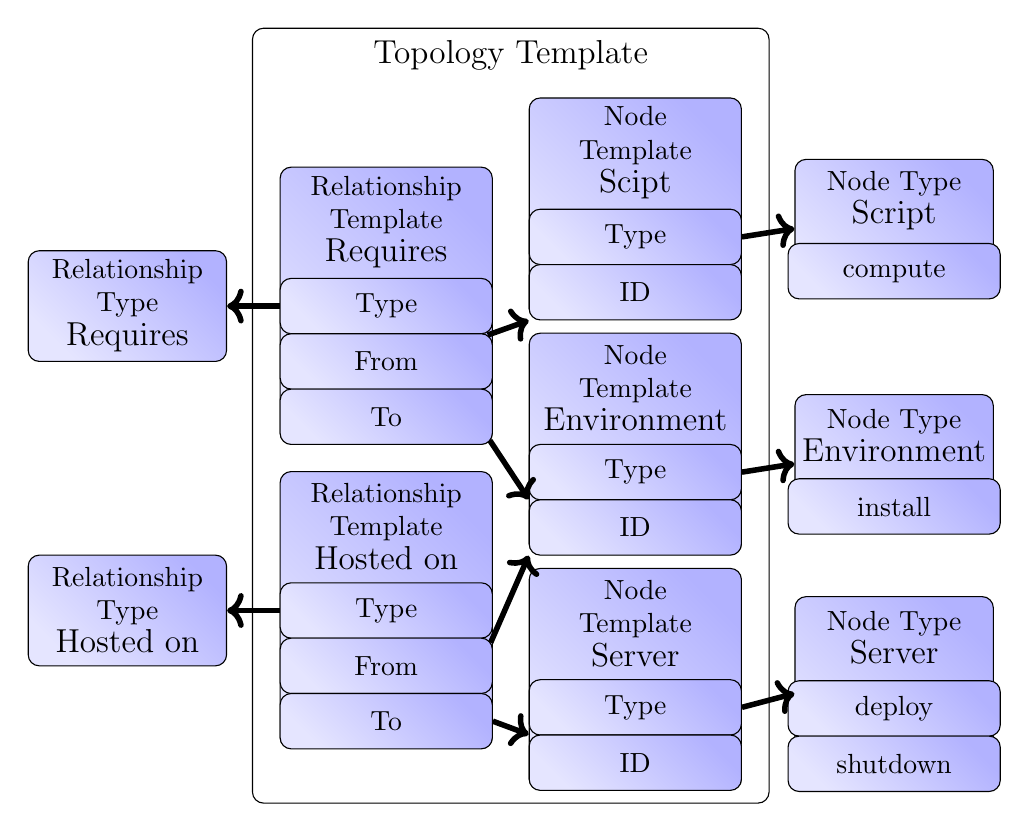
\begin{tikzpicture}
\node (topology) [topology] {};
\node at (topology.north)[yshift=-1em] {\large Topology Template};


\node (requirestemplate) [xshift=-4.5em, yshift=+9em] at ( topology) [rtemplate] {};
\node (requirestemplatetype) at (requirestemplate) [yshift=+1em] [item] {Type};
\node (requirestemplatefrom) at (requirestemplate) [yshift=-1em] [item] {From};
\node (requirestemplateto) at (requirestemplate) [yshift=-3em] [item] {To};
\node at (requirestemplate.north) [yshift=-2em][align=center] {Relationship\\Template\\\large Requires};

\node (hostedtemplate) [xshift=-4.5em, yshift=-2em] at ( topology) [rtemplate] {};
\node (hostedtemplatetype) at (hostedtemplate) [yshift=+1em] [item] {Type};
\node (hostedtemplatefrom) at (hostedtemplate) [yshift=-1em] [item] {From};
\node (hostedtemplateto) at (hostedtemplate) [yshift=-3em] [item] {To};
\node at (hostedtemplate.north) [yshift=-2em][align=center] {Relationship\\Template\\\large Hosted on};

\node (scripttemplate) [xshift=+4.5em, yshift=+11.5em] at ( topology) [ntemplate] {};
\node (scripttemplatetype) at (scripttemplate) [yshift=+0em] [item] {Type};
\node (scripttemplateID) at (scripttemplate) [yshift=-2em] [item] {ID};
\node at (scripttemplate.north) [yshift=-2em][align=center] {Node\\Template\\\large Scipt};

\node (environmenttemplate) [xshift=+4.5em, yshift=+3em] at ( topology) [ntemplate] {};
\node (environmenttemplatetype) at (environmenttemplate) [yshift=+0em] [item] {Type};
\node (environmenttemplateID) at (environmenttemplate) [yshift=-2em] [item] {ID};
\node at (environmenttemplate.north) [yshift=-2em][align=center] {Node\\Template\\\large Environment};

\node (servertemplate) [xshift=+4.5em, yshift=-5.5em] at ( topology) [ntemplate] {};
\node (servertemplatetype) at (servertemplate) [yshift=+0em] [item] {Type};
\node (servertemplateID) at (servertemplate) [yshift=-2em] [item] {ID};
\node at (servertemplate.north) [yshift=-2em][align=center] {Node\\Template\\\large Server};

\node (requirestype) [xshift=-5.5em, yshift=+2em] at ( requirestemplate.west) [rtype] {};
\node at (requirestype.north) [yshift=-2em][align=center] {Relationship\\Type\\\large Requires};

\node (hostedontype) [xshift=-5.5em, yshift=+2em] at ( hostedtemplate.west) [rtype] {};
\node at (hostedontype.north) [yshift=-2em][align=center] {Relationship\\Type\\\large Hosted on};

\node (scripttype) [xshift=+5.5em, yshift=+1.8em] at ( scripttemplate.east) [ntype, minimum height=5em] {};
\node  at (scripttype.south) [yshift=+2em] [item] {compute};
\node at (scripttype.north) [yshift=-1.5em][align=center] {Node Type\\\large Script};

\node (environmenttype) [xshift=+5.5em, yshift=+1.8em] at ( environmenttemplate.east) [ntype, minimum height=5em] {};
\node  at (environmenttype.south) [yshift=+2em] [item] {install};
\node at (environmenttype.north) [yshift=-1.5em][align=center] { Node Type\\\large Environment};

\node (servertype) [xshift=+5.5em, yshift=+3em] at ( servertemplate.east) [ntype] {};
\node  at (servertype.south) [yshift=+4em] [item] {deploy};
\node  at (servertype.south) [yshift=+2em] [item] {shutdown};
\node at (servertype.north) [yshift=-1.5em][align=center] { Node Type\\\large Server};

\draw [->,scale=5,line width=2pt,shorten <= -2pt] (requirestemplatefrom.north east) -- (scripttemplateID.south west);
\draw [->,scale=5,line width=2pt,shorten <= -2pt] (requirestemplateto.south east) -- (environmenttemplateID.north west);
\draw [->,scale=5,line width=2pt,shorten <= -2pt] (hostedtemplatefrom.north east) -- (environmenttemplateID.south west);
\draw [->,scale=5,line width=2pt] (hostedtemplateto.east) -- (servertemplateID.north west);

\draw [->,scale=5,line width=2pt] (requirestemplatetype.west) -- (requirestype.east);
\draw [->,scale=5,line width=2pt] (hostedtemplatetype.west) -- (hostedontype.east);

\draw [->,scale=5,line width=2pt] (servertemplatetype.east) -- (servertype.west);
\draw [->,scale=5,line width=2pt] (environmenttemplatetype.east) -- (environmenttype.west);
\draw [->,scale=5,line width=2pt] (scripttemplatetype.east) -- (scripttype.west);
\end{tikzpicture} 
\caption{Example: a cloud application for weather calculation} 	\label{fig:weather}
\end{figure}
%
\subsection*{CSAR} 
%
To store a TOSCA application a \gls{csar}\label{sec:csar} is used.
This is a ZIP-file with ".csar" extension that contains all the data needed for instantiation and management of TOSCA application.
They include definition documents, artifacts and so on.
In this form, a TOSCA application can be processed by a TOSCA runtime environment.\\
%\subsubsection*{Structure}
The root folder of any CSAR must contain the "Definitions" and "\gls{tosca}-Metadata" folders.
The "Definitions" folder contains definition documents one of which must define a Service Template.
The "\gls{tosca}-Metadata" folder must contain TOSCA metadata in the form of a file with the "TOSCA.meta" name.
This metafile consists of name/value pairs, one line for each pair. 
The first set of pairs describes CSAR itself (TOSCA version, CSAR version, creator and so on). 
All other pairs represent metadata of files from the CSAR. 
The metadata is used by a TOSCA runtime environment to process given files correctly.\\
%
%\subsubsection*{Terms}
%During this work, such terms as input CSAR and output CSAR will be used.
%The input \gls{csar} is the \gls{csar}, which can contain external references and will be processed by the framework. %\\
%The output CSAR is the CSAR, which was processed by the framework and doesn't contain external references. %(at least those that are handled by the framework).
\subsection*{Encapsulation of CSARs}
The encapsulation must be achieved through the download of external packages and generation of a new TOSCA node for each of them. 
But it can be interesting to analyze other techniques to encapsulate a CSAR. 
At first, we will described the methods not representing packages in a TOSCA topology and then the methods mirroring packages into the topology.\\
\subsubsection*{Generate Custom Repositories}
It's possible to download all necessary packages and create one's own custom package repository for each device used in the application. 
Then one must rework any package installation commands or exchange system preferences to setup an access to the custom repository.
This method introduces minimal changes in a TOSCA structure.
The main problem is the creation of the custom repositories. 
When a TOSCA application consists of many small devices with limited capabilities it can be difficult to start many big custom repositories.\\
\subsubsection*{Generate Shared Repository}
Another opportunity is to create a single repository for all devices in a TOSCA application.
It can be difficult to choose the right location for such a server, but since an application represents the connected system this step can redistribute the load to a more powerful device.
It is difficult to estimate the changes which will occur in a TOSCA topology while applying such a method.\\
\subsubsection*{One Node for One Package}
This method was suggested by IAAS. 
A new TOSCA node will be created for each downloaded package. 
All dependencies between packages will be mirrored to a TOSCA topology.
This is a very visual method, facilitating the understanding of a TOSCA application and dependencies between packages.\\
\subsubsection*{Sets of Packages}
A set of depended packages from a dependencies tree related to an external reference can be archived and represented in a TOSCA topology as a single node.
An installation of such a node will lead to the installation of all needed packages.
Of course, some packages can be saved in different archives redundantly, but a small size of a TOSCA application's structure will be achieved.
It will be impossible to trace dependencies (since all packages are represented by one node), but it can help to avoid a difficult structure which consists of hundreds of nodes. \\
\section{OpenTOSCA} \label{sec:opentosca}
OpenTOSCA provides an open source web-based ecosystem for \gls{tosca} applications. 
%It was developed at the University of Stuttgart in october 2012.
This ecosystem consists of three parts: the \gls{tosca} \textbf{runtime environment}, the graphical modeling TOSCA tool \textbf{Winery}, and the self-service portal for the applications available in the container \textbf{Vinothek}.~\cite*{OpenTOSCA}
Descriptions of the runtime environment and Winery will be provided in more detail. 
\subsection*{Runtime Environment}
The runtime environment enables a fully automated plan-based deployment and management of Cloud applications contained in a CSAR. 
The architecture of the environment is visualized by Figure~\ref{fig:openarch}.
Requests to the Container API are passed to the Control component, which orchestrates the different components, tracks their progress, and interprets the TOSCA application. 
The Core component offers common services to other components, e. g., managing data or validating XML.
Management operations of nodes and relationships are either provided by running (Web) services, e. g., the Amazon EC2 API, or by Implementation Artifacts contained in the CSAR.
In the latter case, the Implementation Artifact Engine is responsible to run these artifacts in order to make them available for plans. 
The plugin architecture of the Implementation Artifact Engine ensure extensibility.
Implementation Artifacts, e. g., a SOAP Web service implemented as Java Web archive, are processed by a corresponding plugin of the engine which knows where and how to run this kind of artifact. 
The plugins deploy the respective artifacts and return the endpoints of the deployed management operations to be stored in the Endpoints database.
The deployment of Web Archives on Tomcat~\cite*{tomcat} and Axis Archives on Apache Axis~\cite*{axis} is supported~\cite*{macharb}.
The Plan Engine handles plans in the same manner.
It is also build according to a plugin architecture and supports different workflow languages, e.g., Business Process Model and Notation (BPMN) or Business Process Execution (BPEL) Language, and their runtime environments.~\cite{INPROC-2013-45}
\\
A processing is done in following manner.  
First, the CSAR is unpacked and the files are put into the files store.
Then, the TOSCA definitions documents are loaded, resolved, validated, and processed by the Control component, which calls the Implementation Artifact Engine and the Plan Engine.
The Implementation Artifact Engine deploys the referenced Implementation Artifacts and stores their endpoints in the Endpoints database. 
Finally, the Plan Engine binds and deploys the application’s management plans.
The endpoints of the management plans are stored in the Plans database.~\cite{INPROC-2013-45}
%% !TeX spellcheck = en_US

% We need layers to draw the block diagram
\usetikzlibrary{calc,positioning}
\usetikzlibrary{arrows.meta}

% Define a few styles and constants
\tikzstyle{entry}=[draw, fill=green!20, minimum height=2.5em]
\tikzstyle{ann} = [above, text width=5em]
\tikzstyle{framework} = [entry, text width=30em, fill=white, 
minimum height=20em, rounded corners]
\tikzstyle{lang} = [entry, text width=9em, shading = axis,rectangle, left color=blue!10!white, right color=blue!30!white,shading angle=135, anchor=north,
minimum height=3em, rounded corners]
\tikzstyle{control} = [entry, text width=11em, shading = axis,rectangle, left color=blue!10!white, right color=blue!30!white,shading angle=135, anchor=north,
minimum height=12em, rounded corners]
\tikzstyle{core} = [entry, text width=14em, shading = axis,rectangle, left color=blue!10!white, right color=blue!30!white,shading angle=135, anchor=north,
minimum height=3em, rounded corners]
\tikzstyle{ia} = [entry, text width=9em, shading = axis,rectangle, left color=blue!10!white, right color=blue!30!white,shading angle=135, anchor=north,
minimum height=4em, rounded corners]
\tikzstyle{service} = [entry, text width=9em, shading = axis,rectangle, left color=blue!10!white, right color=blue!30!white,shading angle=135, anchor=north,
minimum height=4em, rounded corners]
\tikzstyle{plan} = [entry, text width=9em, shading = axis,rectangle, left color=blue!10!white, right color=blue!30!white,shading angle=135, anchor=north,
minimum height=4em, rounded corners]
\tikzstyle{item} = [entry, text width=8em, shading = axis,rectangle, left color=blue!20!white, right color=blue!40!white,shading angle=135, anchor=north,
minimum height=1em, rounded corners]
\def\blockdist{2.3}
\def\edgedist{2.5}

\begin{figure}
	\centering
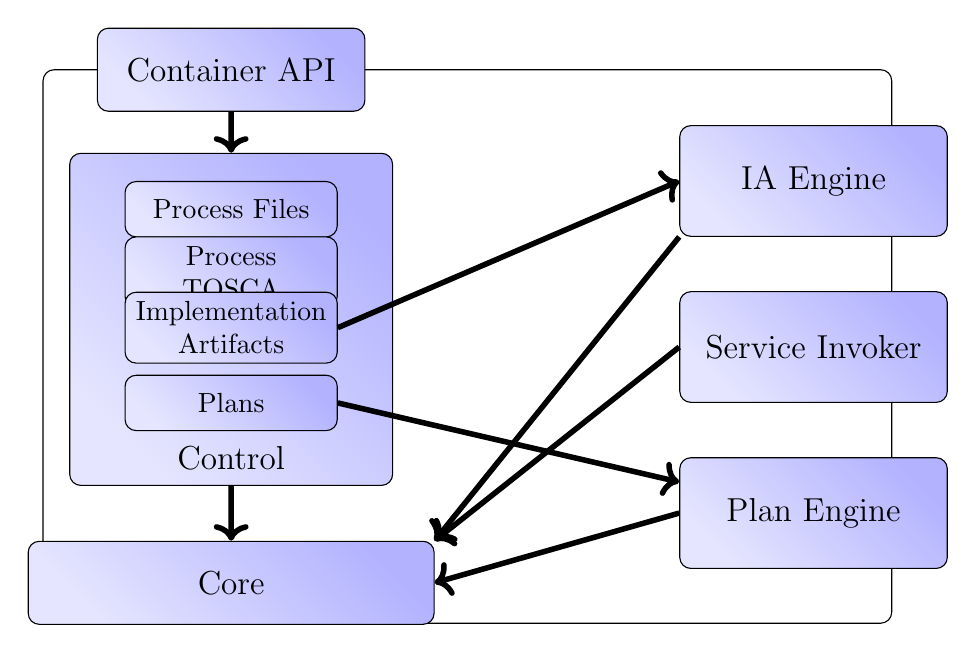
\begin{tikzpicture}
\node (rr) [framework] {};


\node (lang1) [xshift=-30mm, yshift=+1.5em] at ( rr.north) [lang] {};
\node at (lang1) {\large Container API};

\node (control) [xshift=-30mm, yshift=+7em] at ( rr) [control] {};
\node [yshift=+1em] at (control.south) {\large Control};

\node [xshift=-0mm, yshift=+5em] at ( control) [item] {Process Files};
\node [xshift=-0mm, yshift=+3em] at ( control) [item] {Process TOSCA};
\node (impl)[xshift=-0mm, yshift=+1em] at ( control) [item] {Implementation Artifacts};
\node (plans)[xshift=-0mm, yshift=+-2em] at ( control) [item] {Plans};

\node (core) [xshift=-30mm, yshift=+3em] at ( rr.south) [core] {};
\node at (core) {\large Core};

\node (ia) [xshift=-10mm, yshift=+8em] at ( rr.east) [ia] {};
\node at (ia) {\large IA Engine};

\node (service) [xshift=-10mm, yshift=+2em] at ( rr.east) [service] {};
\node at (service) {\large Service Invoker};

\node (plan) [xshift=-10mm, yshift=-4em] at ( rr.east) [plan] {};
\node at (plan) {\large Plan Engine};

\draw [->,scale=5,line width=2pt] (lang1) -- (control);
\draw [->,scale=5,line width=2pt] (control) -- (core);
\draw [->,scale=5,line width=2pt] (plan.west) -- (core.east);
\draw [->,scale=5,line width=2pt] (service.west) -- (core.north east);
\draw [->,scale=5,line width=2pt] (ia.south west) -- (core.north east);
\draw [->,scale=5,line width=2pt] (impl.east) -- (ia.west);
\draw [->,scale=5,line width=2pt] (plans.east) -- (plan);
\end{tikzpicture} 
\caption{OpenTOSCA runtime environment control flow} 	\label{fig:opencontainer}
\end{figure}
% !TeX spellcheck = en_US

% We need layers to draw the block diagram
\usetikzlibrary{calc,positioning}
\usetikzlibrary{arrows.meta}

% Define a few styles and constants
\tikzstyle{entry}=[draw, minimum height=2em, align=center]
\tikzstyle{mytext}=[align=center]
\tikzstyle{frame} = [entry, text width=29em, fill=white,minimum height=20em, rounded corners]
\tikzstyle{db} = [entry, text width=26em, fill=white,minimum height=6em, rounded corners, left color=green!15!white, right color=green!20!white,shading angle=135, anchor=north]
\tikzstyle{dbentry} = [entry, text width=4em, fill=white,minimum height=3em, rounded corners, left color=blue!15!white, right color=blue!20!white,shading angle=135, anchor=north]
\tikzstyle{overbox} = [entry, text width=6em, shading = axis,rectangle, left color=blue!10!white, right color=blue!30!white,shading angle=135, anchor=north,
minimum height=3em, rounded corners]
\tikzstyle{longbox} = [entry, text width=24em, shading = axis,rectangle, left color=orange!15!white, right color=orange!20!white,shading angle=135, anchor=north,
minimum height=2em, rounded corners]
\tikzstyle{shortbox} = [entry, text width=12em, shading = axis,rectangle, left color=orange!15!white, right color=orange!20!white,shading angle=135, anchor=north,
minimum height=2em, rounded corners]
\tikzstyle{intern} = [entry, text width=8em, shading = axis,rectangle, left color=blue!10!white, right color=blue!30!white,shading angle=135, anchor=north,
minimum height=6em, rounded corners]
\tikzstyle{internr} = [entry, text width=17em, shading = axis,rectangle, left color=blue!10!white, right color=blue!30!white,shading angle=135, anchor=north,
minimum height=6em, rounded corners]
\tikzstyle{corned} = [entry, text width=5em, shading = axis,rectangle, left color=blue!10!white, right color=blue!30!white,shading angle=135, anchor=north,
minimum height=2em, rounded corners]
\def\blockdist{2.3}
\def\edgedist{2.5}

\begin{figure}
	\centering
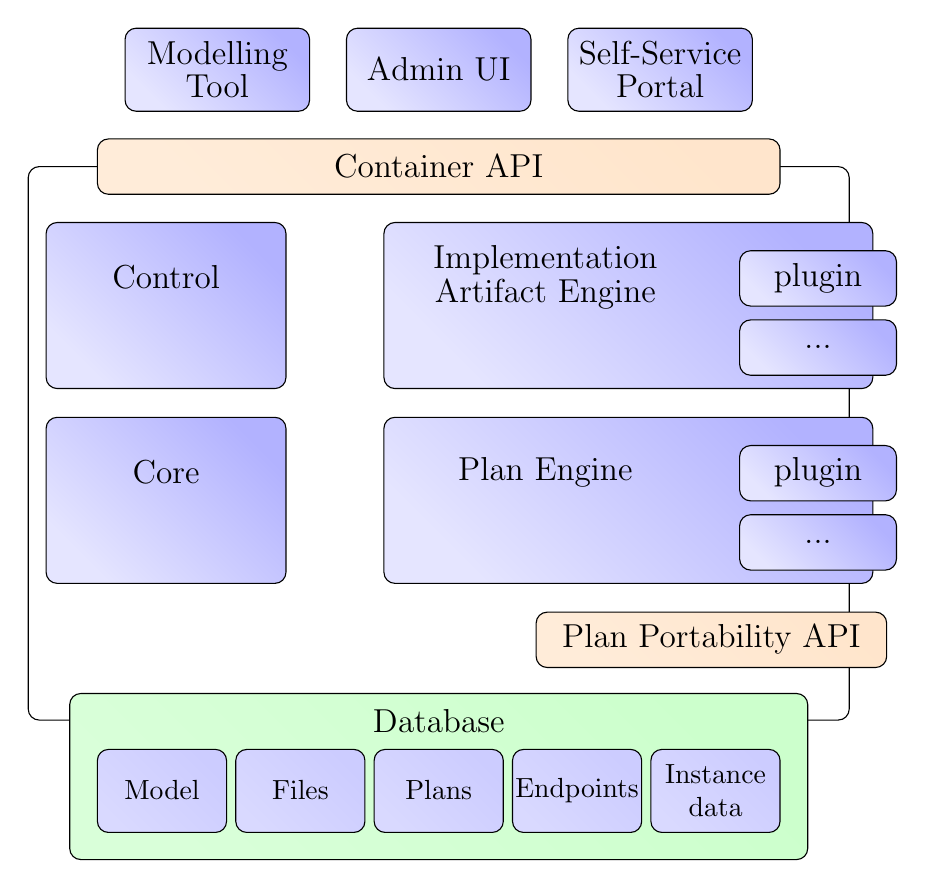
\begin{tikzpicture}
\node (frame) [frame] {};

\node (conapi) [xshift=0em, yshift=+1em] at (frame.north) [longbox] {};
\node at (conapi.north) [yshift=-1em][mytext] {\large Container API};

\node (admininter) [xshift=0em, yshift=+4em] at (conapi.north) [overbox] {};
\node at (admininter.north) [yshift=-1.5em][mytext] {\large Admin UI};

\node (modeltool) [xshift=-8em, yshift=+4em] at (conapi.north) [overbox] {};
\node at (modeltool.north) [yshift=-1.5em][mytext] {\large Modelling\\\large Tool};

\node (selfport) [xshift=+8em, yshift=+4em] at (conapi.north) [overbox] {};
\node at (selfport.north) [yshift=-1.5em][mytext] {\large Self-Service\\\large Portal};

\node (control) [xshift=+5em, yshift=+8em] at (frame.west) [intern] {};
\node at (control.north) [yshift=-2em][mytext] {\large Control};

\node (core) [xshift=+0em, yshift=-1em] at (control.south) [intern] {};
\node at (core.north) [yshift=-2em][mytext] {\large Core};

\node (implart) [xshift=-8em, yshift=8em] at (frame.east) [internr] {};
\node at (implart.north) [xshift=-3em,yshift=-2em][mytext] {\large Implementation\\\large Artifact Engine};

\node (planengine) [xshift=+0em, yshift=-1em] at (implart.south) [internr] {};
\node at (planengine.north) [xshift=-3em,yshift=-2em][mytext] {\large Plan Engine};

\node (pluginimplart) [xshift=-2em, yshift=+2em] at (implart.east) [corned] {};
\node at (pluginimplart.north) [yshift=-1em][mytext] {\large plugin};

\node (dotsimplart) [xshift=-2em, yshift=-0.5em] at (implart.east) [corned] {};
\node at (dotsimplart.north) [yshift=-1em][mytext] {\large ...};

\node (pluginplanengine) [xshift=-2em, yshift=+2em] at (planengine.east) [corned] {};
\node at (pluginplanengine.north) [yshift=-1em][mytext] {\large plugin};

\node (dotsplanengine) [xshift=-2em, yshift=-0.5em] at (planengine.east) [corned] {};
\node at (dotsplanengine.north) [yshift=-1em][mytext] {\large ...};

\node (planport) [xshift=+3em, yshift=-1em] at (planengine.south) [shortbox] {};
\node at (planport.north) [yshift=-1em][mytext] {\large Plan Portability API};

\node (db) [xshift=-0em, yshift=+1em] at (frame.south) [db] {};
\node at (db.north) [yshift=-1em][mytext] {\large Database};

\node (plans) [xshift=-0em, yshift=+1em] at (db) [dbentry] {};
\node at (plans.north) [yshift=-1.5em][mytext] {Plans};

\node (files) [xshift=-5em, yshift=+1em] at (db) [dbentry] {};
\node at (files.north) [yshift=-1.5em][mytext] {Files};

\node (model) [xshift=-10em, yshift=+1em] at (db) [dbentry] {};
\node at (model.north) [yshift=-1.5em][mytext] {Model};

\node (endpoints) [xshift=+5em, yshift=+1em] at (db) [dbentry] {};
\node at (endpoints.north) [yshift=-1.5em][mytext] {Endpoints};

\node (Instancedata) [xshift=+10em, yshift=+1em] at (db) [dbentry] {};
\node at (Instancedata.north) [yshift=-1.5em][mytext] {Instance\\ data};



\end{tikzpicture} 
\caption{OpenTOSCA Architecture} 	\label{fig:openarch}
\end{figure}
\subsection*{Winery}\label{subs:wine}\label{tool:winery}
Winery provides a complete set of functions for graphically create, edit and delete elements in the TOSCA topology presented by a CSAR. 
It consists of four parts: the type and template management, the topology modeler, the BPMN4TOSCA plan modeler ~\cite{BPMN4TOSCA}, and the repository.\\
The type, template and artifact management enables managing all TOSCA types, templates and related artifacts. 
This includes node types, relationship types, policy types, artifact types, artifact templates, and artifacts such as virtual machine images.\\
The topology modeler allows to create service templates which consist of node templates and relationship templates. 
They can be annotated with requirements and capabilities, properties, and policies.\\
BPMN4TOSCA plan modeler offers web-based creation of BPMN models with the TOSCA extension: BPMN4TOSCA. 
That means the modeler supports the BPMN elements and structures required by TOSCA plans and not the full set of BPMN. 
The Stardust project~\cite*{stardust} offers Browser Modeler, which covers all phases of the Business Process Lifecycle including modeling, simulation, execution and monitoring. 
In the context of Winery, this modeler was extended to support BPMN4TOSCA.\\
The repository stores TOSCA models and allows managing their content. 
For instance, node types, policy types, and artifact templates are managed by the repository. 
The repository is also responsible for importing and exporting CSARs, the exchange format of TOSCA files and related artifacts.~\cite{winery} %\\
%Winery works under a Tomcat server and therefore a visual interface is available in a browser. %, example in Figure \ref{fig:winery_gui}.
An example of the TOSCA topology visualization is presented in Figure~\ref{fig:winery_source}.
%\begin{figure}[ht]   
%	\centering
%	\includegraphics[width=0.7\textwidth]{Screenshot_winery_gui.png}
%	\caption{Visual interface for $Winery$.}
%	\label{fig:winery_gui}
%\end{figure}
\begin{figure}[ht]   
\centering
\includegraphics[width=0.7\textwidth]{Screenshot_winery_source.png}
\caption{TOSCA topology visualized by $Winery$.}
\label{fig:winery_source}
\end{figure}
\section{Package Management} \label{sec:pm}
Packages and package management processes are described in this section.
An installation of packages from external source represents an external reference and therefore they will be considered in order to identify such references.
%\subsection*{Package managers}
Package is an archive file containing both data for installation of the program component and a set of metadata like name, function, version, producer, and a list of dependencies to other packages.~\cite*{opium}
These packages can present not only a complete program but also a certain component of a large application. % or libraries, a packages which can be used only by other programs.
For a user, a package manager is a set of software tools which automate the process of installing, updating, configuring and removing packages.
But from the operating system side, a package manager is used for managing the database of packages, their dependencies, and versions, to prevent erroneous installation of programs and missing dependencies.
%\subsection*{Packages}
%\subsection*{Dynamic libraries}
This task is especially complex in computer systems relying on dynamic library linking. 
Those systems share executable libraries of machine instructions across  applications. 
In these systems, complex relationships between different packages requiring different versions of libraries result in a challenge colloquially known as "dependency hell"~\cite*{linuxgeek}.
Good package management is vital to these systems.\\
%\subsection*{Repository}
To give users more control over the kinds of programs that they allow to install on their systems, packages are often downloaded only from a number of software repositories.
In Unix systems, a package manager uses official repositories appropriate for the operating system and the architecture  of device where it's operate, but it's possible to use additional repositories, like third-party repositories or repositories for another architecture.\\
%\subsection*{Dependencies} \label{subs:dep}
Package managers distinguish between two types of dependencies: $required$ and $preRequired$. %\\
Dependency $package1$ \textbf{$required$} $package2$ indicates that the $package2$ must be installed for a proper \textbf{operation} of the $package1$. %\\
Dependency $package1$ \textbf{$preRequired$} $package2$ indicates that the $package2$ must be installed for a proper \textbf{installation} of the $package1$. %\\
%An example for obtaining the dependency list for the Python package is shown in Listing~\ref{lst:dep}.
%\begin{lstlisting}[caption={Example of using $apt$-$cache$ to obtain dependency list for package python}\label{lst:dep},captionpos=t] 
%user@user:~$ apt-cache depends python
%python
%PreDepends: python-minimal
%Depends: python2.7
%Depends: libpython-stdlib
%Conflicts: <python-central>
%Breaks: update-manager-core
%Suggests: python-doc
%Suggests: python-tk
%Replaces: python-dev
%\end{lstlisting}
%\subsection*{Dependency tree}
In these examples, the $package2$ is needed for the $package1$, but the $package2$ itself can require additional packages.
A structure describing all necessary packages and dependencies between them for the given root-package is called a dependency tree. 
The dependency type $required$ can lead to cycles in dependency trees which differs them from the normal tree graph structures.
\subsection*{Example Dependencies Handling}
The $apt$-$get$ package manager will be considered to provide an example of a dependencies handling.
This application is part of \gls{apt} program which uses $dpkg$ application to communicate with an operating system.
The system keeps a database of packages and their condition.
These relations are presented in Figure~\ref{fig:packages}.\\
$apt$-$get$ has many functions: install, remove, update, autoremove, download and so on.
We will consider the install, remove and autoremove operations to present the common algorithms of processing.
When a package manager becomes a $package$ installation command, it builds a dependencies tree for the $package$ and checks the possibility to install these depended packages.
For example, it must check the compatibility with previously installed packages. 
If the check was successful, the $apt$-$get$ downloads and installs the packages starting with the bottom of the tree.
The $package$ is marked in the database as manually installed and all the other packages are marked as automatically installed. 
It will be helpful during the autoremove operation when all automatically installed packages will be checked whether they are still needed.
After installation of packages from the dependencies tree, the $package$ will be ready to work.\\
A $package$ can be deleted during the $remove$ $package$ command.
It happens only if there are no other packages depending on the $package$. 
If the deletion is very important, then these packages can also be removed too to keep the consistency of the database. 
The packages necessary for the $package$ itself will be deleted only by the autoremove command.
% !TeX spellcheck = en_US

% We need layers to draw the block diagram
\usetikzlibrary{calc,positioning}
\usetikzlibrary{arrows.meta}

% Define a few styles and constants
\tikzstyle{entry}=[draw, fill=green!20, minimum height=2.5em]
\tikzstyle{ann} = [above, text width=5em]
\tikzstyle{item} = [entry, text width=7em, shading = axis,rectangle, left color=blue!10!white, right color=blue!30!white,shading angle=135, anchor=north,
minimum height=2em, rounded corners, align=center]
%\def\blockdist{2.3}
%\def\edgedist{2.5}

\begin{figure}
	\centering
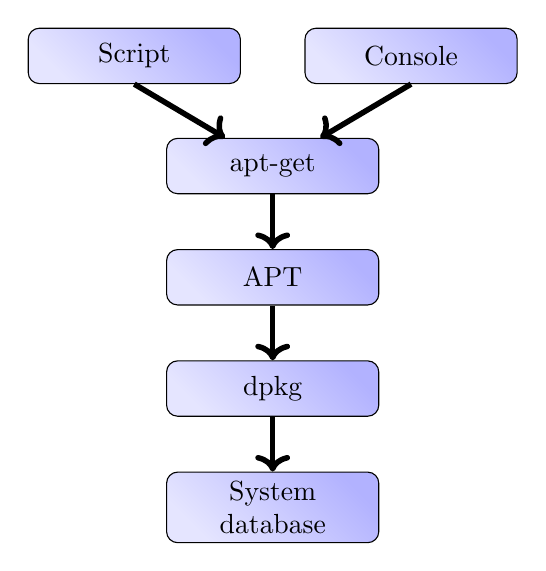
\begin{tikzpicture}
\node (aptget) [item] {apt-get};
\node (console) [yshift=+5em, xshift=+5em] at ( aptget) [item] {Console};
\node (script) [yshift=+5em, xshift=-5em] at ( aptget) [item] {Script};
\node (apt) [yshift=-3em] at ( aptget) [item] {APT};
\node (dpkg) [yshift=-3em] at (apt) [item] {dpkg};
\node (system) [yshift=-3em] at (dpkg) [item] {System database};

\draw [->,scale=1,line width=2pt] (console.south) -- (aptget);
\draw [->,scale=2,line width=2pt] (script.south) -- (aptget);
\draw [->,scale=2,line width=2pt] (aptget) -- (apt);
\draw [->,scale=2,line width=2pt] (apt) -- (dpkg);
\draw [->,scale=2,line width=2pt] (dpkg) -- (system);
\end{tikzpicture} 
\caption{Package management} 	\label{fig:packages}
\end{figure}
\section{Configuration Management Tools}
To ease the package management, various tools can be used. 
We will consider some of them to determine the form of files which contains external references.
Usually they are presented by commands in an executable file, which checks an environment and installs the necessary packages using a package manager.
Such files are called scripts and are commonly used.
Popular management tools like Bash, Ansible, Chef and CFEngine will be described below.
\subsection*{Bash} \label{lang:bash}
Bash is a Unix command language written as a free software.
It provides enough capabilities to be used as a  management tool.
In addition Bash denotes a command processor that typically runs in a text window, where a user types commands that cause actions.
Bash is examined because it is very popular since it is the default command line processor in Unix systems~\cite*{bashdef}.
Instead of typing commands direct into a command line, a script can be executed directly.~\cite{bash}
These scripts can be used to configure a system, install package, create files, check environment and so on.
Bash is a very popular and ease language, therefore a huge number of problems have solutions in Bash scripts already.
\subsection*{Ansible} \label{lang:ansible}
Ansible is an open-source automation engine that automates software provisioning, configuration management, and application deployment.
As with most configuration management software, Ansible has two types of servers: controlling machines and nodes.
First, there is a single controlling machine which is where orchestration begins.
Nodes are managed by a controlling machine over SSH.
The controlling machine describes the location of nodes through its inventory.
Ansible playbooks express configurations, deployment, and orchestration in Ansible.
The playbook format is YAML. 
Each playbook maps a group of hosts to a set of roles.
Each role is represented by calls to Ansible tasks.~\cite{ansible} 
\subsection*{Chef} \label{lang:shef}
Chef is a configuration management tool, which uses Ruby for writing system configuration files called "recipes".
They describe how Chef manages applications and utilities and how they are to be configured.
These recipes which can be grouped together as a "cookbook" for easier management define a series of resources that should be in a particular state: packages that should be installed, services that should be running, or files that should be written.
Chef can run in client/server mode, or in a standalone configuration named "chef-solo".
In client/server mode, the Chef client sends various attributes about the node to the Chef server. 
In solo mode the local system will be configured.~\cite{chef}
\subsection*{CFEngine}
CFEngine is an open source configuration management system.
Its primary function is to provide automated configuration and maintenance of large-scale computer systems, including the unified management of servers, desktops, consumer and industrial devices, embedded networked devices, mobile smartphones, and tablet computers.~\cite{cfengine}
Configurations are described by "policy" files, which are plain text-files with .cf extension.
These files define the necessary state of files, packages, users, processes, services and so on.~\cite{cfengine2}
